\documentclass[a4paper,12pt]{article}
\usepackage{times}
\usepackage[utf8]{inputenc}

\usepackage{graphicx}
\usepackage[english]{babel}
\usepackage[a4paper,includehead]{geometry}
\usepackage{amsmath, amssymb, amsfonts}
\usepackage{subcaption}
\usepackage[numbers,square,sort&compress]{natbib}
\usepackage{adjustbox}
\geometry{left=19mm,right=19mm,top=18.5mm,bottom=20mm}
\setlength{\parindent}{0cm}
\setlength{\parskip}{0.3cm}
\usepackage{enumitem}
\usepackage{caption}
\usepackage{hyperref}
\usepackage{tabularx}
\usepackage{booktabs}
\usepackage{tikz}
\usetikzlibrary{positioning, fit, arrows.meta, backgrounds}
\captionsetup{labelfont=bf}
 \hypersetup{
     colorlinks=true,
     linkcolor=blue,
     filecolor=blue,
     citecolor = red,      
     urlcolor=purple,
     }
\usepackage{booktabs}
\usepackage{threeparttable}
\usepackage{multicol}
\usepackage{multirow}
\usepackage{listings}
\usepackage[acronym, nonumberlist]{glossaries}
\usepackage{comment}
\usepackage{float}




\setitemize{itemsep=5pt,topsep=0pt,parsep=0pt,partopsep=0pt}
\linespread{1.1}

\usepackage{minted}

\usepackage{mathtools}

\usepackage{booktabs}
\usepackage{tabularx}
\newcolumntype{L}{>{\raggedright\arraybackslash}X}

\usepackage{tcolorbox}
\usepackage{environ}

\newif\ifshowboxes
\showboxestrue

\NewEnviron{mybox}{
    \ifshowboxes
        \begin{tcolorbox}
        \BODY
        \end{tcolorbox}
    \fi
}
\showboxesfalse

% \usepackage{geometry}

% % Set the margins automatically
% \geometry{
%   margin=auto,
% }

% \usepackage{geometry}

% % Set the margins here
% \geometry{
%   left=1cm,
%   right=1cm,
%   top=2cm,
%   bottom=2cm,
% }



\begin{document}
\begin{titlepage}
\newcommand{\HRule}{\rule{\linewidth}{0.5mm}} % Defines a new command for the horizontal lines, change thickness here
\center % Center everything on the page
 
%----------------------------------------------------------------------------------------
%	HEADING SECTIONS
%----------------------------------------------------------------------------------------

\textsc{\LARGE Katholieke Universiteit Leuven}\\[0.5cm] % Name of your university/college
\vspace{1cm}
\includegraphics[scale=0.2]{logo_kul.jpeg}\\[1cm] % Include a department/university logo - this will require the graphicx package
\vspace{1cm}
\textsc{Privacy and Big Data (B-KUL-H00Y2B)}\\[0.2cm] % Major heading such as course name


%----------------------------------------------------------------------------------------
%	TITLE SECTION
%----------------------------------------------------------------------------------------

\HRule \\[0.4cm]
{ \huge \bfseries Privacy impact assessment: FitBuddy }\\[0.1cm] % Title of your document
\HRule \\[1.2cm]

%----------------------------------------------------------------------------------------
%	AUTHOR SECTION
%----------------------------------------------------------------------------------------

\begin{minipage}{0.48\textwidth}
    \begin{flushleft}
        Storm Van Dooren r0945564 \\
        Lars Vansweevelt r0947252 \\
        Laurens Van Goethem r1038575\\
        Michel Moussally r0913670\\
    \end{flushleft}
\end{minipage}
\begin{minipage}{0.48\textwidth}
    \begin{flushright}
    \emph{Professor:} \\
    Prof. Galvez Vizcaino Rafa
    
    \emph{Supervisor:} \\

    \end{flushright}
    \end{minipage}\\[1.5cm]


% If you don't want a supervisor, uncomment the two lines below and remove the section above
%\Large \emph{Author:}\\
%John \textsc{Smith}\\[3cm] % Your name

%----------------------------------------------------------------------------------------
%	DATE SECTION
%----------------------------------------------------------------------------------------
\vspace{0.5cm}
{\large \today}\\[1.5cm] % Date, change the \today to a set date if you want to be precise
\vfill % Fill the rest of the page with whitespace
\end{titlepage}
\pagebreak

    \newpage
    \thispagestyle{empty}
    \tableofcontents
    \newpage
    \pagenumbering{arabic}




\section{Application Description}
\label{sec:application}

FitBuddy is a free, open-source health tracker for Android, released under the GNU General
Public License v3.0 by a single developer~\cite{fitbuddy-repo}. We assess version 3.2.82 (commit
\texttt{28d1adb}). Unless another source is cited, all statements about the implementation were
verified in this source code~\cite{fitbuddy-repo}. Where the code does not reveal how a
component behaves, we state our assumptions explicitly in Section~\ref{sec:assumptions}.

\subsection{Access to the Application}
\begin{itemize}
  \item Source code: \url{https://github.com/anantdark/FitBuddy}~\cite{fitbuddy-repo}
  \item F-Droid page: \url{https://f-droid.org/en/packages/com.anant.fitbuddy/}~\cite{fitbuddy-fdroid}
\end{itemize}
The app is distributed in two \emph{build flavours} built from the same code: a GitHub build,
published on GitHub Releases, and an F-Droid build. They differ in their crash-reporting
default, update source and signing key.

\subsection{Functionality}
Users log meals and workouts by taking a photo or typing a free-text description. A large
language model (LLM) estimates the calories and macronutrients, after which the user reviews the
estimate, adjusts ingredient weights and saves it. Packaged foods can be scanned by barcode and
looked up in Open Food Facts~\cite{off-api}. Further features are a daily dashboard, reusable
meal presets, structured workouts with an exercise catalog~\cite{exercisedb-repo},
body-measurement tracking, progress charts, and an AI ``coach'' that comments on the user's
progress. \emph{Region packs} adapt prompts and staple foods to India, North America, Europe or
Latin America.

During onboarding, the user must connect an AI provider and enter their first and last name,
age, height, weight, optional sex, activity level and goal. Calorie targets are computed on the
device; the AI only picks one of several pre-computed plans.

\subsection{Stakeholders}
Figure~\ref{fig:stakeholders} shows the stakeholders and how they relate to the application.
\begin{itemize}
  \item \textbf{Users} are the data subjects. They also choose the AI provider and create their
        own API key, so they hold the contract with that provider themselves. Users who donate
        become \emph{supporters} and may appear on a public supporter list.
  \item \textbf{The developer} writes and releases the app, but also operates the server-side
        services (a Sentry project, a proxy on Vercel and a MongoDB Atlas database) and develops
        the companion app FreeScale~\cite{freescale-repo}. For telemetry and cloud backups, the
        developer determines the purposes and means of processing and therefore acts as
        controller in the sense of Art.~4(7) GDPR~\cite{gdpr}.
  \item \textbf{AI providers} (OpenRouter, Google Gemini, Ollama~\cite{ollama}, OpenAI or any
        compatible host) receive photos, descriptions and profile data. With a self-hosted
        Ollama server, the user is their own provider.
  \item \textbf{Processors and platforms}: Sentry~\cite{sentry-android}, Vercel~\cite{vercel}
        and MongoDB Atlas~\cite{mongodb-atlas} process data on behalf of the developer; Google
        stores the Android backup~\cite{android-autobackup}; GitHub and F-Droid distribute the
        app and serve update information.
  \item \textbf{Public data services}: Open Food Facts~\cite{off-api} (product data) and the
        jsDelivr CDN~\cite{jsdelivr} (exercise catalog and images).
\end{itemize}
Roles overlap: Google is both a possible AI provider (Gemini) and the backup host, GitHub hosts
both the code and the supporter list, and the developer is involved on both sides of the
FreeScale interface.

\begin{figure}[htbp]
\centering
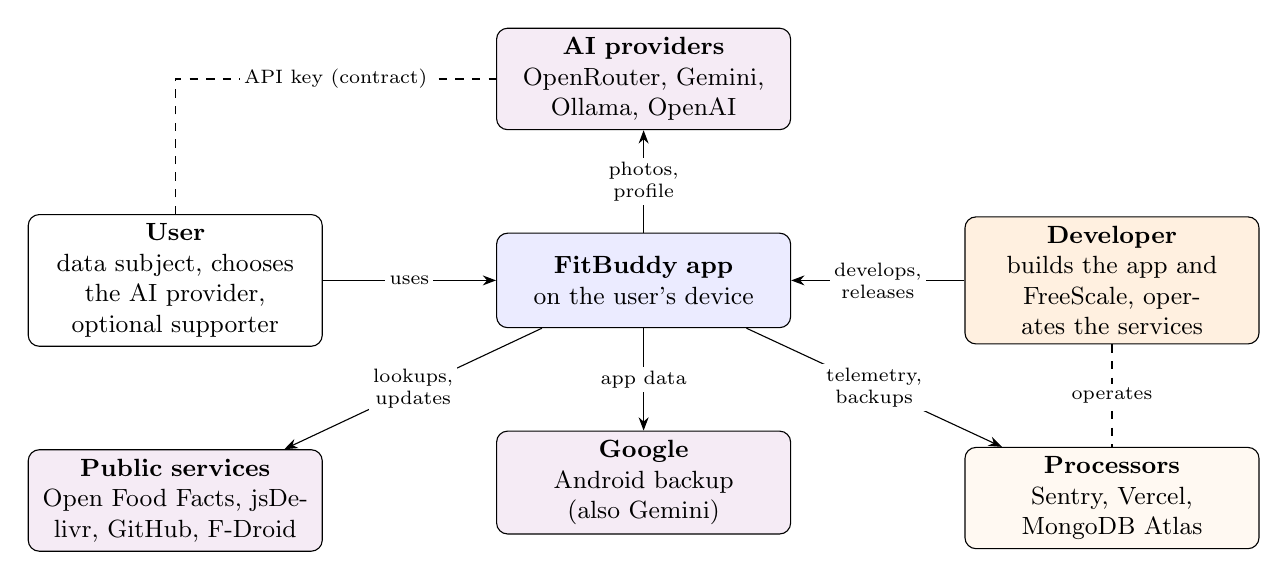
\begin{tikzpicture}[
    font=\small,
    box/.style={draw, rounded corners, align=center, text width=3.5cm, minimum height=1.2cm},
    lbl/.style={font=\scriptsize, fill=white, inner sep=1.5pt, align=center},
    >=Stealth
  ]
  \node[box, fill=blue!8] (app) {\textbf{FitBuddy app}\\on the user's device};
  \node[box, left=2.2cm of app] (user) {\textbf{User}\\data subject, chooses the AI provider, optional supporter};
  \node[box, right=2.2cm of app, fill=orange!12] (dev) {\textbf{Developer}\\builds the app and FreeScale, operates the services};
  \node[box, above=1.3cm of app, fill=violet!8] (ai) {\textbf{AI providers}\\OpenRouter, Gemini, Ollama, OpenAI};
  \node[box, below=1.3cm of app, fill=violet!8] (google) {\textbf{Google}\\Android backup (also Gemini)};
  \node[box, below=1.3cm of dev, fill=orange!5] (proc) {\textbf{Processors}\\Sentry, Vercel, MongoDB Atlas};
  \node[box, below=1.3cm of user, fill=violet!8] (pub) {\textbf{Public services}\\Open Food Facts, jsDelivr, GitHub, F-Droid};

  \draw[->] (user) -- node[lbl] {uses} (app);
  \draw[->] (dev) -- node[lbl] {develops,\\releases} (app);
  \draw[->] (app) -- node[lbl] {photos,\\profile} (ai);
  \draw[->] (app) -- node[lbl] {app data} (google);
  \draw[->] (app) -- node[lbl] {telemetry,\\backups} (proc);
  \draw[->] (app) -- node[lbl] {lookups,\\updates} (pub);
  \draw[dashed] (user) |- node[lbl, pos=0.75] {API key (contract)} (ai);
  \draw[dashed] (dev) -- node[lbl] {operates} (proc);
\end{tikzpicture}
\caption{Stakeholders of FitBuddy. Solid arrows show data or software flows; dashed lines show
contractual or operational relations. Purple: independent third parties; orange: the developer
and the services they operate.}
\label{fig:stakeholders}
\end{figure}

\subsection{Collected Data and Purposes}
Table~\ref{tab:data} lists the personal data that FitBuddy processes, why, and where it goes.
Body measurements, dietary and activity records are \emph{data concerning health}
(Art.~4(15) GDPR), and the region can indicate ethnic or cultural background; both are special
categories of personal data under Art.~9 GDPR~\cite{gdpr}.

\begin{table}[htbp]
\centering
\footnotesize
\caption{Personal data processed by FitBuddy. Flow numbers refer to Figure~\ref{fig:architecture}.}
\label{tab:data}
\begin{tabularx}{\textwidth}{@{}L L l@{}}
\toprule
\textbf{Data} & \textbf{Purpose} & \textbf{Leaves the device via} \\
\midrule
First and last name & Personalised greeting; usage statistics for the developer & 2, 5 \\
Age, sex, height, weight, activity level, goal & Calorie targets; context for AI estimates & 1, 2, 6, 7 \\
Body measurements (weight, body fat, BMR, muscle mass, further smart-scale values) & Progress
  tracking & 1, 2, 6--8 \\
Meals, ingredients, scanned barcodes, presets & Core logging function & 2, 3, 6, 7, 9 \\
Meal photos and free-text descriptions & AI estimation; not stored on the device & 1 \\
Workouts and exercise logs & Core logging function & 2, 6, 7, 9 \\
Region & Adapting prompts and foods; revealed by the regional prompts & 1, 2 \\
Support ID (random UUID) & Identifies cloud backups and crash reports & 5, 6 \\
Device model, name and identifier & Crash diagnosis and usage statistics; labelling backups & 5, 6 \\
AI API keys & Authenticating to the chosen AI provider & 1, 2, 6, 7 \\
\bottomrule
\end{tabularx}
\end{table}

FitBuddy requests no location, contacts or storage permissions; the only sensitive permission is
the camera, and gallery images are selected with the system photo picker~\cite{android-photopicker}.
Photos are re-encoded before upload, which removes EXIF metadata such as GPS coordinates.

\subsection{Architecture}
Figure~\ref{fig:architecture} shows the architecture at an abstract level. The app is written in
Kotlin with a Jetpack Compose user interface~\cite{android-compose} and follows a layered design:
a user interface, application logic, and local storage consisting of a SQLite database accessed
through Room~\cite{android-room} for health records and a key--value store (Android
DataStore~\cite{android-datastore}) for settings, identifiers and API keys. There is no user
account and no central application server. All communication with external parties is
summarised as flows (1)--(9).

\begin{figure}[htbp]
  \centering
  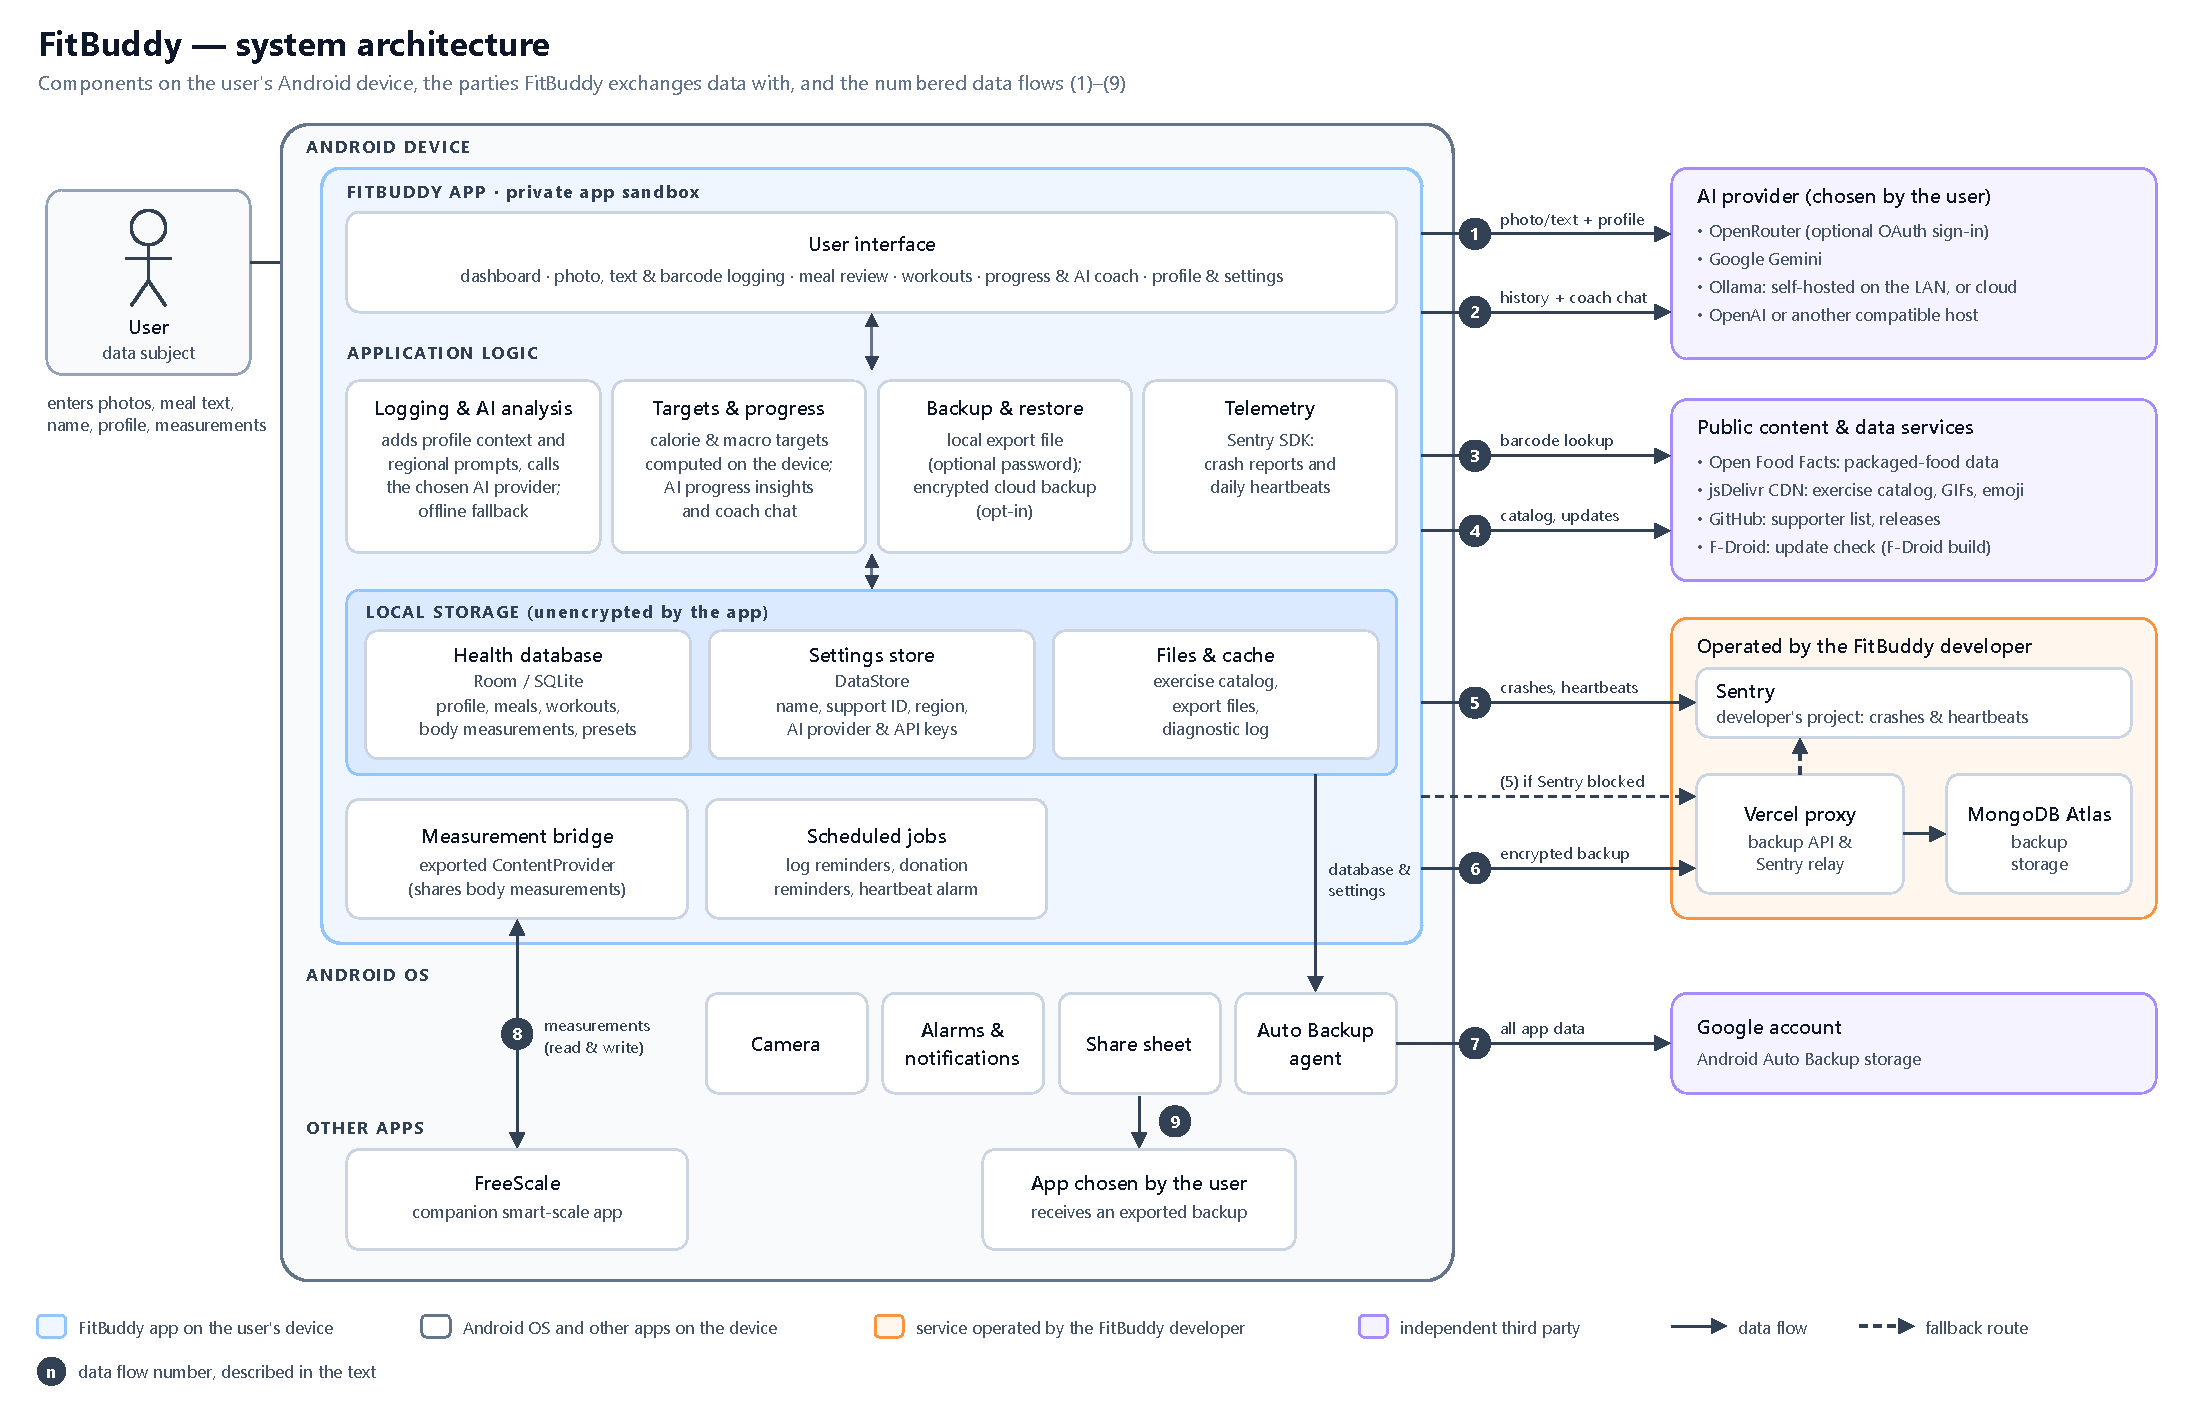
\includegraphics[width=\textwidth]{fitbuddy_architecture.pdf}
  \caption{Abstract architecture of FitBuddy and its data flows: (1) AI estimation, (2) progress
  insights and coach chat, (3) barcode lookup, (4) catalog and update requests, (5) telemetry,
  (6) cloud backup, (7) Android Auto Backup, (8) measurement exchange with FreeScale, (9) manual
  export.}
  \label{fig:architecture}
\end{figure}

\subsection{Design and Implementation Choices}
\subsubsection{Local-first storage}
All records stay on the device and can be deleted individually; there is no option to delete all
data at once. The app adds no encryption of its own and relies on Android's file-based
encryption~\cite{android-fbe}.

\subsubsection{Bring your own AI provider}
Each AI request (flow 1) contains the photo or text plus a summary of the profile, today's
calorie balance and the latest body measurement. Progress insights (flow 2) add 30 days of
detailed history, monthly averages of older data and the first name. The user selects the
provider; with a self-hosted Ollama server, the data stays in the user's own network, which is
why unencrypted HTTP is allowed for user-configured servers. Failover between API keys and
models never switches to another provider.

\subsubsection{Telemetry}
The app uses the Sentry SDK~\cite{sentry-android} for crash reports, configured without IP
addresses and with a filter for secrets. Crash reporting is on by default in the GitHub build
without asking, and off by default in the F-Droid build. Independently of this setting, a daily
and post-update \emph{heartbeat} reports the user's full name, the date of their first log, the
number of records, the AI provider and the device model. When Sentry is unreachable, for example
because of a DNS-based blocker, telemetry is relayed through the developer's Vercel proxy.

\subsubsection{Backups}
Three backup mechanisms exist. Android Auto Backup~\cite{android-autobackup} copies all app data,
including API keys, to the user's Google account (flow 7). An optional cloud backup (flow 6)
uploads an encrypted copy of all data to MongoDB Atlas through the developer's proxy,
automatically at most every 12 hours. It uses AES-256 in Galois/Counter Mode~\cite{nist-gcm}
with a key derived by PBKDF2~\cite{rfc8018} from a user-chosen password or, by default, from the
support ID; the backup is stored and retrieved under that same ID and cannot be deleted from the
app. Finally, users can export a backup file, which is unencrypted unless a password is set
(flow 9).

\subsubsection{Integration with other apps}
The measurement bridge is an exported Android content provider~\cite{android-contentprovider}
that lets FreeScale read all measurements and add new ones (flow 8). It accepts callers based on
their package name.

\subsubsection{Other choices}
Barcodes are decoded on the device; only the barcode is sent to Open Food Facts (flow 3). The
OpenRouter sign-in uses OAuth with PKCE~\cite{openrouter-oauth,rfc7636}.

\subsection{Assumptions}
\label{sec:assumptions}
\begin{itemize}
  \item The server-side code of the developer's Vercel proxy is not public. We assume it stores
        backups unchanged in MongoDB Atlas and forwards telemetry to Sentry without further
        processing.
  \item We treat the AI providers, Sentry, Google and Open Food Facts as black boxes that process
        the received data according to their own policies; their retention periods are not
        considered.
  \item We consider a typical user in the European Union who installs the GitHub build and uses a
        cloud-hosted AI provider. The companion app FreeScale is out of scope apart from its
        interface with FitBuddy.
\end{itemize}



\section{LINDDUN Threat Model}
\label{sec:threat-model}

We follow the LINDDUN PRO methodology~\cite{linddun-pro}: we first model the system as a data
flow diagram (DFD) with trust boundaries, derived from the architecture in
Figure~\ref{fig:architecture}. We then define the information at risk, our trust assumptions
and the potential adversaries, and finally elicit threats for each of the seven LINDDUN threat
types~\cite{linddun-types,deng2011}. The prioritisation of these threats follows in
Section~\ref{sec:privacy-issues}.

\subsection{Data Flow Diagram}
Figure~\ref{fig:dfd} shows the DFD. It uses the four element types of LINDDUN: external
entities (E), processes (P), data stores (DS) and data flows~\cite{linddun-pro}. The flow numbers
are the same as in Figure~\ref{fig:architecture}.

\begin{figure}[htbp]
\centering
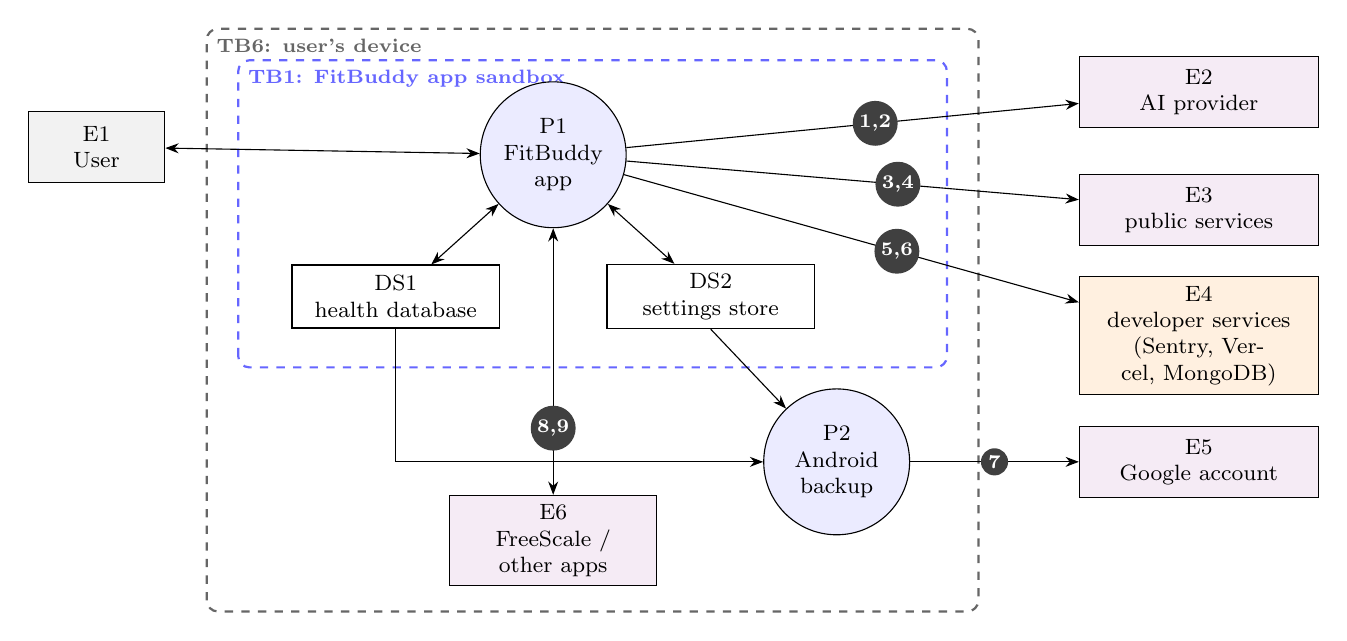
\begin{tikzpicture}[
    font=\footnotesize, >=Stealth,
    ext/.style={draw, fill=violet!8, align=center, text width=2.8cm, minimum height=0.9cm},
    dev/.style={draw, fill=orange!12, align=center, text width=2.8cm, minimum height=0.9cm},
    usr/.style={draw, fill=gray!10, align=center, text width=1.5cm, minimum height=0.9cm},
    proc/.style={circle, draw, fill=blue!8, align=center, text width=1.5cm, inner sep=1pt},
    ds/.style={draw, fill=white, align=center, text width=2.4cm, minimum height=0.8cm},
    num/.style={circle, fill=black!75, text=white, font=\scriptsize\bfseries, inner sep=1.2pt},
    tb/.style={draw, dashed, thick, rounded corners}
  ]
  % trust boundaries
  \draw[tb, black!60] (0.6,-3.1) rectangle (10.4,4.3);
  \node[anchor=north west, font=\scriptsize\bfseries, text=black!60] at (0.6,4.3) {TB6: user's device};
  \draw[tb, blue!60] (1.0,0.0) rectangle (10.0,3.9);
  \node[anchor=north west, font=\scriptsize\bfseries, text=blue!60] at (1.0,3.9) {TB1: FitBuddy app sandbox};

  % elements
  \node[usr] (e1) at (-0.8,2.8) {E1\\User};
  \node[proc] (p1) at (5,2.7) {P1\\FitBuddy app};
  \node[ds] (ds1) at (3,0.9) {DS1\\health database};
  \node[ds] (ds2) at (7,0.9) {DS2\\settings store};
  \node[proc] (p2) at (8.6,-1.2) {P2\\Android backup};
  \node[ext, text width=2.4cm] (e6) at (5,-2.2) {E6\\FreeScale / other apps};
  \node[ext] (e2) at (13.2,3.5) {E2\\AI provider};
  \node[ext] (e3) at (13.2,2.0) {E3\\public services};
  \node[dev] (e4) at (13.2,0.4) {E4\\developer services\\(Sentry, Vercel, MongoDB)};
  \node[ext] (e5) at (13.2,-1.2) {E5\\Google account};

  % flows
  \draw[<->] (e1) -- (p1);
  \draw[<->] (p1) -- (ds1);
  \draw[<->] (p1) -- (ds2);
  \draw[->] (p1) -- node[num, pos=0.55] {1,2} (e2);
  \draw[->] (p1) -- node[num, pos=0.6] {3,4} (e3);
  \draw[->] (p1) -- node[num, pos=0.6] {5,6} (e4);
  \draw[->] (ds2.south) -- (p2);
  \draw[->] (ds1.south) |- (p2.west);
  \draw[->] (p2) -- node[num, pos=0.5] {7} (e5);
  \draw[<->] (p1) -- node[num, pos=0.75] {8,9} (e6);
\end{tikzpicture}
\caption{LINDDUN data flow diagram of FitBuddy with trust boundaries TB1 (app sandbox) and TB6
(device). Every arrow that leaves TB6 crosses a further trust boundary (TB2--TB5, see
Section~\ref{sec:trust}). Purple: independent third parties; orange: services operated by the
developer.}
\label{fig:dfd}
\end{figure}

\subsection{Information at Risk}
Table~\ref{tab:assets} summarises the assets. The main risk is \emph{aggregation}: single records
reveal little, but together they form a longitudinal health profile that the identifiers in A3
link to a named person.

\begin{table}[htbp]
\centering
\footnotesize
\caption{Information at risk.}
\label{tab:assets}
\begin{tabularx}{\textwidth}{@{}l L l L@{}}
\toprule
\textbf{ID} & \textbf{Asset} & \textbf{Stored / flows} & \textbf{Sensitivity} \\
\midrule
A1 & Health profile and body measurements & DS1; 1, 2, 6--8 & Art.~9 GDPR~\cite{gdpr} \\
A2 & Meal and workout history, meal photos & DS1; 1--3, 6, 7, 9 & Art.~9; may reveal illness, religion or eating disorders \\
A3 & Full name, support ID, device name and identifier & DS2; 5, 6 & Links all other assets to a person \\
A4 & AI provider API keys & DS2; 1, 2, 6, 7 & Financial abuse; access to provider-side history \\
A5 & Region, progress insights, coach conversations & 1, 2 & Region may reveal ethnic origin (Art.~9) \\
\bottomrule
\end{tabularx}
\end{table}

\subsection{Trust Assumptions and Trust Boundaries}
\label{sec:trust}
\subsubsection{Trust assumptions}
\begin{description}[style=nextline, leftmargin=0.6cm]
  \item[TA1 -- Android platform.] The OS sandbox and Keystore work as specified and the device is
    not rooted, so other apps can only reach FitBuddy's data through exported components.
  \item[TA2 -- Transport security.] TLS to HTTPS endpoints is sound. This does not hold for
    user-configured servers, because cleartext HTTP is allowed application-wide.
  \item[TA3 -- AI providers are semi-honest.] They follow the protocol and return correct
    estimates, but may analyse and retain what they receive~\cite{goldreich2004}. Their terms
    govern further use; Google's unpaid Gemini tier, for example, uses submitted content to
    improve its products, allows human review and asks users not to submit personal
    information~\cite{gemini-terms}.
  \item[TA4 -- The developer and their processors are semi-honest.] We assume no malicious
    intent, but the developer can read everything sent in plaintext, and their infrastructure can
    be breached. The key that authorises requests to the backup proxy is embedded in every copy
    of the app and must therefore be considered public.
  \item[TA5 -- Google backup.] The Auto Backup is end-to-end encrypted only on Android~9 or
    later with a screen lock~\cite{android-autobackup}; otherwise its confidentiality depends on
    the user's Google account.
  \item[TA6 -- Out of scope.] Compromise of the build pipeline or libraries, and attacks on the
    language models themselves.
\end{description}

\subsubsection{Trust boundaries}
\begin{description}[style=nextline, leftmargin=0.6cm]
  \item[TB1 -- App sandbox $\leftrightarrow$ other apps (flows 8, 9).] The measurement bridge
    accepts callers by package name only; exports go to any app the user picks.
  \item[TB2 -- Device $\leftrightarrow$ AI provider (flows 1, 2).] The main boundary for health
    data. For self-hosted servers, the local network also lies on this boundary.
  \item[TB3 -- Device $\leftrightarrow$ developer services (flows 5, 6).] Crossed daily without
    user interaction. Because telemetry is rerouted when Sentry is blocked, the user's own
    network filters do not enforce this boundary.
  \item[TB4 -- Device $\leftrightarrow$ Google (flow 7).] Crossed by the OS, outside the app's
    control.
  \item[TB5 -- Device $\leftrightarrow$ public services (flows 3, 4).] Only queries and the IP
    address cross it, but barcodes reveal which products the user eats.
  \item[TB6 -- Device $\leftrightarrow$ person holding it.] Data at rest is not encrypted by the
    app.
\end{description}

\subsection{Potential Adversaries}
Table~\ref{tab:adversaries} lists the adversaries. The most capable ones are not outsiders but
parties that receive data \emph{by design} (ADV3, ADV4), and anyone who learns a support ID
(ADV6): the app asks users to share this ID when reporting a bug, while it also serves as the
default backup password.

\begin{table}[htbp]
\centering
\footnotesize
\caption{Potential adversaries.}
\label{tab:adversaries}
\begin{tabularx}{\textwidth}{@{}l l L l l@{}}
\toprule
\textbf{ID} & \textbf{Adversary} & \textbf{Capability} & \textbf{TB} & \textbf{Assets} \\
\midrule
ADV1 & Network attacker & HTTPS: metadata only. Cleartext LAN servers: read and modify photos,
  profile and API keys & 2, 5 & A1, A2, A4 \\
ADV2 & Malicious app & Installed under FreeScale's package name while FreeScale is absent:
  read and inject measurements & 1 & A1 \\
ADV3 & AI provider & Receives every photo with profile context; retains or trains on it & 2
  & A1, A2, A5 \\
ADV4 & Developer & Receives full names daily; can decrypt backups without a custom password & 3
  & A1--A5 \\
ADV5 & Attacker on developer services & As ADV4, for all users at once & 3 & A1--A5 \\
ADV6 & Support-ID holder & Downloads the backup with the public proxy key and decrypts it if no
  password was set & 3 & A1--A5 \\
ADV7 & Physical or account access & Reads the unencrypted database and keys, or restores the
  Google backup elsewhere & 4, 6 & A1--A5 \\
ADV8 & Public service & Links IP address to scanned products & 5 & A2 \\
\bottomrule
\end{tabularx}
\end{table}

\subsection{LINDDUN Threat Elicitation}
Following LINDDUN PRO, we iterated over each interaction in Figure~\ref{fig:dfd} and considered
the source, the flow and the destination~\cite{linddun-pro}. Table~\ref{tab:linddun} lists the
resulting threats per threat type, as defined in~\cite{linddun-types}.

\begin{table}[htbp]
\centering
\footnotesize
\caption{Elicited privacy threats per LINDDUN threat type.}
\label{tab:linddun}
\begin{tabularx}{\textwidth}{@{}l L l@{}}
\toprule
\textbf{ID} & \textbf{Threat} & \textbf{DFD elements} \\
\midrule
\multicolumn{3}{@{}l}{\textit{Linking}} \\
L1 & The support ID links crash reports, heartbeats and backups of one user across services & DF5, DF6, E4 \\
L2 & The public supporter list contains the SHA-256 hash of supporters' support IDs, linking a
     named supporter to their telemetry and backups & E3, E4 \\
\multicolumn{3}{@{}l}{\textit{Identifying}} \\
I1 & Daily heartbeats contain the user's first and last name & DF5, E4 \\
I2 & Backups carry the user-defined device name, which often contains the owner's name, and a
     device identifier & DF6, E4 \\
\multicolumn{3}{@{}l}{\textit{Non-repudiation}} \\
NR1 & Timestamped meal and weight records in backups can serve as evidence, e.g.\ of fasting or
      pregnancy, comparable to the LINDDUN example of menstruation apps~\cite{linddun-types} & DS1, DF6, DF7 \\
\multicolumn{3}{@{}l}{\textit{Detecting}} \\
D1 & The timing of requests to the AI provider reveals when the user eats & DF1 \\
D2 & Heartbeats reveal daily app usage and the number of records & DF5 \\
\multicolumn{3}{@{}l}{\textit{Data disclosure}} \\
DD1 & Every AI request includes profile and body data not needed for the estimate & DF1, DF2, E2 \\
DD2 & The default backup key is derived from the support ID, which is sent along with the backup & DF6, E4 \\
DD3 & No encryption at rest; exports are plaintext unless a password is set & DS1, DS2, DF9 \\
DD4 & API keys are included in the Google backup and in cloud backups & DF6, DF7 \\
DD5 & Cleartext HTTP to self-hosted servers exposes data on the local network & DF1, DF2 \\
DD6 & The measurement bridge does not verify the caller's signing certificate & DF8, E6 \\
\multicolumn{3}{@{}l}{\textit{Unawareness and unintervenability}} \\
U1 & Heartbeats are sent even after opting out of crash reports, although the crash-reporting
     screen states that names are never sent; the GitHub build enables crash reports without
     asking & DF5 \\
U2 & Users are not shown which profile data accompanies each AI request & DF1, DF2 \\
U3 & There is no option to delete all data, and cloud backups cannot be deleted & DS1, E4 \\
\multicolumn{3}{@{}l}{\textit{Non-compliance}} \\
NC1 & No privacy policy and no explicit consent for processing health data (Art.~9(2)(a)
      GDPR~\cite{gdpr}) & P1, E2, E4 \\
NC2 & Telemetry is relayed around user-installed blockers & DF5, E4 \\
\bottomrule
\end{tabularx}
\end{table}

\section{Privacy Issues}
\label{sec:privacy-issues}

The LINDDUN analysis in Section~\ref{sec:threat-model} yielded 18 threats. In this section we
group them into concrete privacy issues, prioritise them, and discuss the most important ones in
detail. All issues were confirmed in the source code~\cite{fitbuddy-repo}.

\subsection{Prioritisation Criteria}
LINDDUN PRO leaves prioritisation to the analyst, suggesting that likelihood and impact be
assessed while taking into account the type and number of data subjects and the sensitivity of
the data~\cite{linddun-pro}. We score both on a scale from 1 (low) to 3 (high):
\begin{itemize}
  \item \textbf{Impact}: the sensitivity of the exposed data (Art.~9 data scores highest), the
        number of affected users, and whether the exposure contradicts what users are told.
  \item \textbf{Likelihood}: whether the issue occurs by default for every user or requires an
        opt-in or unusual configuration, and how much effort the adversary needs.
\end{itemize}
The risk is the product of both scores; ties are broken by impact. Table~\ref{tab:issues}
shows the result.

\begin{table}[htbp]
\centering
\footnotesize
\caption{Privacy issues ordered by risk (I = impact, L = likelihood, R = I $\times$ L).
Threat IDs refer to Table~\ref{tab:linddun}, adversaries to Table~\ref{tab:adversaries}.}
\label{tab:issues}
\begin{tabularx}{\textwidth}{@{}c L l l c c c@{}}
\toprule
\textbf{\#} & \textbf{Issue} & \textbf{Threats} & \textbf{Adversaries} & \textbf{I} & \textbf{L} & \textbf{R} \\
\midrule
1 & Health profile sent with every AI request & DD1, U2, NC1 & ADV3 & 3 & 3 & 9 \\
2 & Cloud backups protected by a shareable identifier & DD2, DD4, L1 & ADV4--6 & 3 & 2 & 6 \\
3 & Named telemetry despite opt-out & I1, D2, U1, NC2 & ADV4, ADV5 & 2 & 3 & 6 \\
4 & No complete erasure & U3, NR1 & ADV4--7 & 2 & 2 & 4 \\
5 & Unprotected local copies & DD3, DD4 & ADV7 & 3 & 1 & 3 \\
6 & Cleartext traffic to self-hosted servers & DD5 & ADV1 & 3 & 1 & 3 \\
7 & Measurement bridge trusts package names & DD6 & ADV2 & 2 & 1 & 2 \\
8 & Linkable identifiers and queries & L2, I2, D1 & ADV4, ADV8 & 2 & 1 & 2 \\
\bottomrule
\end{tabularx}
\end{table}

\subsection{Health Profile Sent with Every AI Request}
\label{sec:issue-ai}
FitBuddy cannot be set up without an AI provider, so this issue affects every user. Estimating
the calories of a photographed meal does not require knowing who ate it, yet each request
(flow~1) carries the user's age, sex, height, weight, goal, activity level, calorie targets,
today's intake and expenditure, and the latest body-fat percentage, basal metabolic rate and
muscle mass. Progress insights and the coach (flow~2) add the user's first name, 30 days of daily
nutrition, exercise and body data, and monthly averages of the entire history. Over time, the
provider thus receives a detailed, timestamped health profile.

By default, FitBuddy uses OpenRouter with free models, and paid OpenRouter and Gemini models are
hidden unless the user enables ``show paid models''. Such tiers may use submitted content for product improvement: Google's unpaid Gemini
API allows human reviewers to read inputs and explicitly asks users not to submit personal
information~\cite{gemini-terms}. FitBuddy never shows which data accompanies a request (U2), has
no privacy policy, and does not ask for the explicit consent that Art.~9(2)(a) GDPR requires for
health data~\cite{gdpr}. Although users choose the provider, the app decides what is sent, which
violates the data-minimisation principle of Art.~5(1)(c) GDPR~\cite{gdpr}.

\subsection{Cloud Backups Protected by a Shareable Identifier}
\label{sec:issue-backup}
When a user enables cloud backup without choosing a password, the encryption key is derived from
the support ID (Listing~\ref{lst:backup-key}). The AES-256-GCM encryption therefore protects the
backup only as long as the support ID is secret, but it is not:
\begin{itemize}
  \item the backup is stored at \texttt{/api/backup/\{supportId\}}, so the developer and anyone who
        breaches the database (ADV4, ADV5) hold the key next to the ciphertext;
  \item the support ID is attached to every crash report as the Sentry user ID;
  \item the app asks users to ``share this if you report a bug''.
\end{itemize}
Access control at the proxy does not compensate for this: the proxy accepts a single API key that
is shared by all installations. It is stored XOR-obfuscated in \texttt{build.gradle.kts}, together
with the mask, in the public repository, so anyone can decode it. An adversary who learns a
support ID (ADV6) can thus download the backup with the same request the app uses for restoring
and decrypt it. The backup contains the complete health history and all API keys (DD4). The issue
requires the opt-in cloud backup, but the password is optional and the settings screen only
describes the support ID as a ``document key''.

\begin{lstlisting}[language=Java, basicstyle=\ttfamily\footnotesize, frame=single,
  caption={Passphrase selection for cloud backups in \texttt{FitnessRepository.kt} (simplified).},
  label={lst:backup-key}, captionpos=b]
if (settings.cloudBackupPasswordSet) return decryptedUserPassword
return supportId.toCharArray()   // default: the support ID is the passphrase
\end{lstlisting}

\subsection{Named Telemetry Despite Opt-out}
\label{sec:issue-telemetry}
Every day, and after each update, FitBuddy sends a heartbeat to the developer's Sentry project
containing the user's first and last name (mandatory during onboarding), the date of their first
log, the number of records, the AI provider and the device model (I1, D2). Contrary to what the
app tells its users, this happens:
\begin{itemize}
  \item \textbf{after opting out.} The code explicitly states that heartbeats are sent
        ``regardless'' of the crash-reporting setting, while the settings screen describes them
        as part of the crash reports, as ``anonymous'', and as something the user can ``turn off
        anytime'';
  \item \textbf{in both builds.} The F-Droid build disables crash reports by default and shows a
        screen promising that ``nothing about your meals, photos, name, or API keys is ever
        sent'', yet heartbeats with the user's name are still sent. In the GitHub build, crash
        reporting is additionally switched on without asking;
  \item \textbf{around blockers.} If Sentry is unreachable, for example because the user blocks
        it with a DNS filter, the app relays the data through the developer's Vercel proxy
        (NC2). This fallback was introduced in a commit titled ``internal networking reliability
        tweaks'', whose prefix keeps it out of the user-facing changelog.
\end{itemize}
Combined with the support ID (L1), these heartbeats let the developer link a named person to
their crash reports and backups. Since usage statistics do not require a name, and the user
cannot refuse them, this processing lacks a valid legal basis and transparency (Art.~5(1)(a)
and~6 GDPR~\cite{gdpr}).

\subsection{No Complete Erasure}
\label{sec:issue-erasure}
Users can delete individual records, but FitBuddy offers no way to erase all data. Cloud backups
are append-only chunk chains and the app has no function to delete them, so health data persists
on the developer's servers after the user stops using the app. Together with the timestamped
records (NR1), this undermines the right to erasure (Art.~17 GDPR~\cite{gdpr}).

\subsection{Other Issues}
\label{sec:issue-other}
The remaining issues have a lower likelihood because they require physical access, a specific
configuration or a malicious app:
\begin{itemize}
  \item \textbf{Unprotected local copies (5).} Neither the database nor the settings store is
        encrypted by the app, exports are plaintext unless a password is set, and the Google
        backup deliberately includes the API keys~\cite{android-autobackup}.
  \item \textbf{Cleartext traffic (6).} Cleartext HTTP is allowed for the whole app, so photos,
        profile data and API keys sent to a self-hosted server can be read on the local network.
  \item \textbf{Measurement bridge (7).} The exported content provider checks only the caller's
        package name. A malicious app installed under FreeScale's package name, when FreeScale
        itself is absent, can read all measurements and insert false ones.
  \item \textbf{Linkable identifiers (8).} The public supporter list contains SHA-256 hashes of
        supporters' support IDs, backups carry the user-defined device name, and barcode lookups
        reveal the user's IP address to Open Food Facts.
\end{itemize}

\section{Tests}
\label{sec:tests}

We captured issues 1--3 of Table~\ref{tab:issues} in automated tests. Following the Helios
assessment, we extended the project's own test suite rather than building a separate tool: five
JUnit~4~\cite{junit4} tests in a new package \texttt{privacy} under \texttt{app/src/test}, which
run on the JVM with Robolectric~\cite{robolectric}. The application code itself was not changed.
Each test asserts the privacy-preserving behaviour, so it fails until the corresponding
recommendation is implemented, and its failure message names the issue and report section. The
project's continuous integration already runs this test task on every push~\cite{fitbuddy-repo},
so the developers are informed automatically as long as an issue is unresolved.

\subsection{Test Design}
Table~\ref{tab:tests} lists the tests. Each targets a component and data flow of
Figure~\ref{fig:architecture}. The backup tests are security tests, but they protect a privacy
property: the confidentiality of the user's health data in the backup held by the developer.

\begin{table}[htbp]
\centering
\footnotesize
\caption{Privacy tests and the condition under which each passes.}
\label{tab:tests}
\begin{tabularx}{\textwidth}{@{}l c l L@{}}
\toprule
\textbf{Test} & \textbf{Issue} & \textbf{Flow} & \textbf{Passes when} \\
\midrule
\texttt{mealEstimateRequest\_doesNotDiscloseBody\-CompositionOrName} & 1 & 1
  & A meal-estimation request contains no body-fat percentage, BMR, muscle mass or first name \\
\texttt{cloudBackupKey\_isNotDerivedFromSupportId} & 2 & 6
  & Without a user password, the backup key is not the support ID \\
\texttt{backupPayload\_doesNotContainAiApiKeys} & 2 & 6
  & The backup payload contains no AI API keys \\
\texttt{heartbeat\_isNotSent\_afterOptingOut\-OfCrashReports} & 3 & 5
  & After opting out, no telemetry connection is attempted \\
\texttt{heartbeat\_carriesNoPersonalName} & 3 & 5
  & The heartbeat has no name field \\
\bottomrule
\end{tabularx}
\end{table}

The tests drive the production code wherever possible; the first one logs a meal through the
real ViewModel and repository and inspects the request handed to the AI interface. A helper
routes all connections to a local proxy that records and refuses them, so no test data reaches a
real server. Because cloud uploads are disabled in debug builds, the only variant with unit
tests, the backup-key test calls the upload's private passphrase selection directly. Notably, an
existing test, \texttt{CloudUploadEncryptionContractTest}, asserts that a backup \emph{can} be
decrypted with the support ID, and thus locks in issue~2.

\subsection{Results}
The tests are run with
\texttt{./gradlew :app:testGithubDebugUnitTest --tests "com.anant.fitbuddy.privacy.*"}.
As shown in Figure~\ref{fig:test-results}, all five tests fail on version 3.2.82. The telemetry
test also confirms the bypass described in Section~\ref{sec:issue-telemetry}: with crash
reporting disabled, the app first tried to reach Sentry and, after that connection was refused,
the developer's Vercel proxy.

\begin{figure}[htbp]
  \centering
  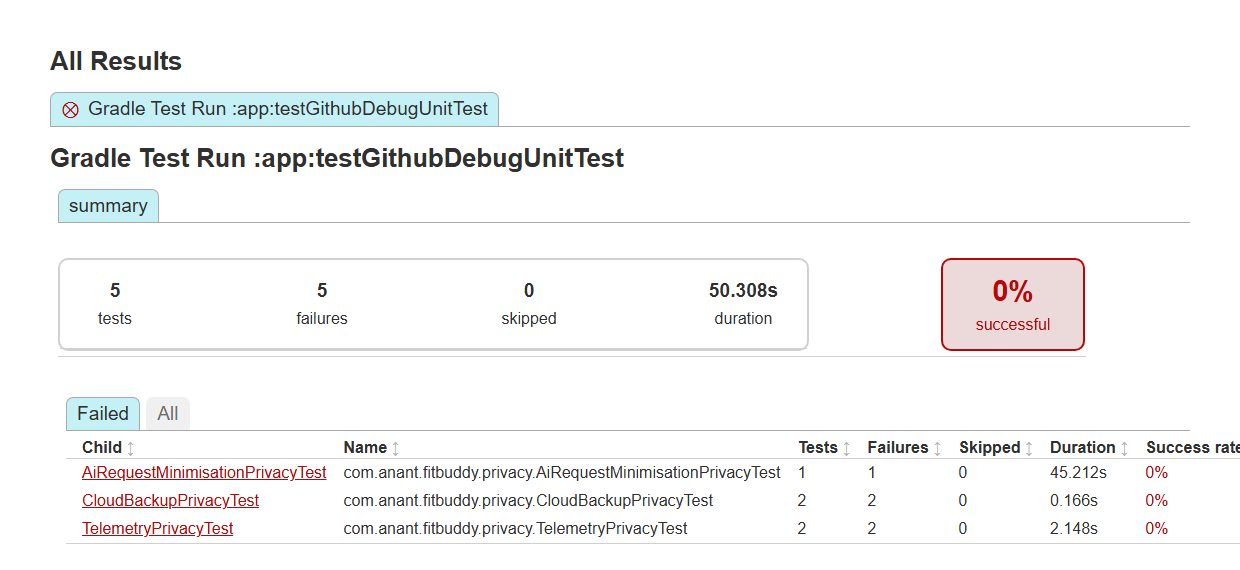
\includegraphics[width=\textwidth]{privacy_tests_report.png}
  \caption{Gradle test report for the privacy tests on FitBuddy 3.2.82: all five tests fail
  because none of the issues has been fixed.}
  \label{fig:test-results}
\end{figure}

\section{Recommendations}

\section{Conclusion}


\newpage
\bibliographystyle{IEEEtran}
\bibliography{reference}

\end{document}

